% Options for packages loaded elsewhere
% Options for packages loaded elsewhere
\PassOptionsToPackage{unicode}{hyperref}
\PassOptionsToPackage{hyphens}{url}
\PassOptionsToPackage{dvipsnames,svgnames,x11names}{xcolor}
%
\documentclass[
  spanish,
  letterpaper,
  DIV=11,
  numbers=noendperiod]{scrartcl}
\usepackage{xcolor}
\usepackage{amsmath,amssymb}
\setcounter{secnumdepth}{-\maxdimen} % remove section numbering
\usepackage{iftex}
\ifPDFTeX
  \usepackage[T1]{fontenc}
  \usepackage[utf8]{inputenc}
  \usepackage{textcomp} % provide euro and other symbols
\else % if luatex or xetex
  \usepackage{unicode-math} % this also loads fontspec
  \defaultfontfeatures{Scale=MatchLowercase}
  \defaultfontfeatures[\rmfamily]{Ligatures=TeX,Scale=1}
\fi
\usepackage{lmodern}
\ifPDFTeX\else
  % xetex/luatex font selection
\fi
% Use upquote if available, for straight quotes in verbatim environments
\IfFileExists{upquote.sty}{\usepackage{upquote}}{}
\IfFileExists{microtype.sty}{% use microtype if available
  \usepackage[]{microtype}
  \UseMicrotypeSet[protrusion]{basicmath} % disable protrusion for tt fonts
}{}
\makeatletter
\@ifundefined{KOMAClassName}{% if non-KOMA class
  \IfFileExists{parskip.sty}{%
    \usepackage{parskip}
  }{% else
    \setlength{\parindent}{0pt}
    \setlength{\parskip}{6pt plus 2pt minus 1pt}}
}{% if KOMA class
  \KOMAoptions{parskip=half}}
\makeatother
% Make \paragraph and \subparagraph free-standing
\makeatletter
\ifx\paragraph\undefined\else
  \let\oldparagraph\paragraph
  \renewcommand{\paragraph}{
    \@ifstar
      \xxxParagraphStar
      \xxxParagraphNoStar
  }
  \newcommand{\xxxParagraphStar}[1]{\oldparagraph*{#1}\mbox{}}
  \newcommand{\xxxParagraphNoStar}[1]{\oldparagraph{#1}\mbox{}}
\fi
\ifx\subparagraph\undefined\else
  \let\oldsubparagraph\subparagraph
  \renewcommand{\subparagraph}{
    \@ifstar
      \xxxSubParagraphStar
      \xxxSubParagraphNoStar
  }
  \newcommand{\xxxSubParagraphStar}[1]{\oldsubparagraph*{#1}\mbox{}}
  \newcommand{\xxxSubParagraphNoStar}[1]{\oldsubparagraph{#1}\mbox{}}
\fi
\makeatother

\usepackage{color}
\usepackage{fancyvrb}
\newcommand{\VerbBar}{|}
\newcommand{\VERB}{\Verb[commandchars=\\\{\}]}
\DefineVerbatimEnvironment{Highlighting}{Verbatim}{commandchars=\\\{\}}
% Add ',fontsize=\small' for more characters per line
\usepackage{framed}
\definecolor{shadecolor}{RGB}{241,243,245}
\newenvironment{Shaded}{\begin{snugshade}}{\end{snugshade}}
\newcommand{\AlertTok}[1]{\textcolor[rgb]{0.68,0.00,0.00}{#1}}
\newcommand{\AnnotationTok}[1]{\textcolor[rgb]{0.37,0.37,0.37}{#1}}
\newcommand{\AttributeTok}[1]{\textcolor[rgb]{0.40,0.45,0.13}{#1}}
\newcommand{\BaseNTok}[1]{\textcolor[rgb]{0.68,0.00,0.00}{#1}}
\newcommand{\BuiltInTok}[1]{\textcolor[rgb]{0.00,0.23,0.31}{#1}}
\newcommand{\CharTok}[1]{\textcolor[rgb]{0.13,0.47,0.30}{#1}}
\newcommand{\CommentTok}[1]{\textcolor[rgb]{0.37,0.37,0.37}{#1}}
\newcommand{\CommentVarTok}[1]{\textcolor[rgb]{0.37,0.37,0.37}{\textit{#1}}}
\newcommand{\ConstantTok}[1]{\textcolor[rgb]{0.56,0.35,0.01}{#1}}
\newcommand{\ControlFlowTok}[1]{\textcolor[rgb]{0.00,0.23,0.31}{\textbf{#1}}}
\newcommand{\DataTypeTok}[1]{\textcolor[rgb]{0.68,0.00,0.00}{#1}}
\newcommand{\DecValTok}[1]{\textcolor[rgb]{0.68,0.00,0.00}{#1}}
\newcommand{\DocumentationTok}[1]{\textcolor[rgb]{0.37,0.37,0.37}{\textit{#1}}}
\newcommand{\ErrorTok}[1]{\textcolor[rgb]{0.68,0.00,0.00}{#1}}
\newcommand{\ExtensionTok}[1]{\textcolor[rgb]{0.00,0.23,0.31}{#1}}
\newcommand{\FloatTok}[1]{\textcolor[rgb]{0.68,0.00,0.00}{#1}}
\newcommand{\FunctionTok}[1]{\textcolor[rgb]{0.28,0.35,0.67}{#1}}
\newcommand{\ImportTok}[1]{\textcolor[rgb]{0.00,0.46,0.62}{#1}}
\newcommand{\InformationTok}[1]{\textcolor[rgb]{0.37,0.37,0.37}{#1}}
\newcommand{\KeywordTok}[1]{\textcolor[rgb]{0.00,0.23,0.31}{\textbf{#1}}}
\newcommand{\NormalTok}[1]{\textcolor[rgb]{0.00,0.23,0.31}{#1}}
\newcommand{\OperatorTok}[1]{\textcolor[rgb]{0.37,0.37,0.37}{#1}}
\newcommand{\OtherTok}[1]{\textcolor[rgb]{0.00,0.23,0.31}{#1}}
\newcommand{\PreprocessorTok}[1]{\textcolor[rgb]{0.68,0.00,0.00}{#1}}
\newcommand{\RegionMarkerTok}[1]{\textcolor[rgb]{0.00,0.23,0.31}{#1}}
\newcommand{\SpecialCharTok}[1]{\textcolor[rgb]{0.37,0.37,0.37}{#1}}
\newcommand{\SpecialStringTok}[1]{\textcolor[rgb]{0.13,0.47,0.30}{#1}}
\newcommand{\StringTok}[1]{\textcolor[rgb]{0.13,0.47,0.30}{#1}}
\newcommand{\VariableTok}[1]{\textcolor[rgb]{0.07,0.07,0.07}{#1}}
\newcommand{\VerbatimStringTok}[1]{\textcolor[rgb]{0.13,0.47,0.30}{#1}}
\newcommand{\WarningTok}[1]{\textcolor[rgb]{0.37,0.37,0.37}{\textit{#1}}}

\usepackage{longtable,booktabs,array}
\usepackage{calc} % for calculating minipage widths
% Correct order of tables after \paragraph or \subparagraph
\usepackage{etoolbox}
\makeatletter
\patchcmd\longtable{\par}{\if@noskipsec\mbox{}\fi\par}{}{}
\makeatother
% Allow footnotes in longtable head/foot
\IfFileExists{footnotehyper.sty}{\usepackage{footnotehyper}}{\usepackage{footnote}}
\makesavenoteenv{longtable}
\usepackage{graphicx}
\makeatletter
\newsavebox\pandoc@box
\newcommand*\pandocbounded[1]{% scales image to fit in text height/width
  \sbox\pandoc@box{#1}%
  \Gscale@div\@tempa{\textheight}{\dimexpr\ht\pandoc@box+\dp\pandoc@box\relax}%
  \Gscale@div\@tempb{\linewidth}{\wd\pandoc@box}%
  \ifdim\@tempb\p@<\@tempa\p@\let\@tempa\@tempb\fi% select the smaller of both
  \ifdim\@tempa\p@<\p@\scalebox{\@tempa}{\usebox\pandoc@box}%
  \else\usebox{\pandoc@box}%
  \fi%
}
% Set default figure placement to htbp
\def\fps@figure{htbp}
\makeatother



\ifLuaTeX
\usepackage[bidi=basic]{babel}
\else
\usepackage[bidi=default]{babel}
\fi
% get rid of language-specific shorthands (see #6817):
\let\LanguageShortHands\languageshorthands
\def\languageshorthands#1{}


\setlength{\emergencystretch}{3em} % prevent overfull lines

\providecommand{\tightlist}{%
  \setlength{\itemsep}{0pt}\setlength{\parskip}{0pt}}



 


\KOMAoption{captions}{tableheading}
\makeatletter
\@ifpackageloaded{tcolorbox}{}{\usepackage[skins,breakable]{tcolorbox}}
\@ifpackageloaded{fontawesome5}{}{\usepackage{fontawesome5}}
\definecolor{quarto-callout-color}{HTML}{909090}
\definecolor{quarto-callout-note-color}{HTML}{0758E5}
\definecolor{quarto-callout-important-color}{HTML}{CC1914}
\definecolor{quarto-callout-warning-color}{HTML}{EB9113}
\definecolor{quarto-callout-tip-color}{HTML}{00A047}
\definecolor{quarto-callout-caution-color}{HTML}{FC5300}
\definecolor{quarto-callout-color-frame}{HTML}{acacac}
\definecolor{quarto-callout-note-color-frame}{HTML}{4582ec}
\definecolor{quarto-callout-important-color-frame}{HTML}{d9534f}
\definecolor{quarto-callout-warning-color-frame}{HTML}{f0ad4e}
\definecolor{quarto-callout-tip-color-frame}{HTML}{02b875}
\definecolor{quarto-callout-caution-color-frame}{HTML}{fd7e14}
\makeatother
\makeatletter
\@ifpackageloaded{caption}{}{\usepackage{caption}}
\AtBeginDocument{%
\ifdefined\contentsname
  \renewcommand*\contentsname{Tabla de contenidos}
\else
  \newcommand\contentsname{Tabla de contenidos}
\fi
\ifdefined\listfigurename
  \renewcommand*\listfigurename{Listado de Figuras}
\else
  \newcommand\listfigurename{Listado de Figuras}
\fi
\ifdefined\listtablename
  \renewcommand*\listtablename{Listado de Tablas}
\else
  \newcommand\listtablename{Listado de Tablas}
\fi
\ifdefined\figurename
  \renewcommand*\figurename{Figura}
\else
  \newcommand\figurename{Figura}
\fi
\ifdefined\tablename
  \renewcommand*\tablename{Tabla}
\else
  \newcommand\tablename{Tabla}
\fi
}
\@ifpackageloaded{float}{}{\usepackage{float}}
\floatstyle{ruled}
\@ifundefined{c@chapter}{\newfloat{codelisting}{h}{lop}}{\newfloat{codelisting}{h}{lop}[chapter]}
\floatname{codelisting}{Listado}
\newcommand*\listoflistings{\listof{codelisting}{Listado de Listados}}
\makeatother
\makeatletter
\makeatother
\makeatletter
\@ifpackageloaded{caption}{}{\usepackage{caption}}
\@ifpackageloaded{subcaption}{}{\usepackage{subcaption}}
\makeatother
\usepackage{bookmark}
\IfFileExists{xurl.sty}{\usepackage{xurl}}{} % add URL line breaks if available
\urlstyle{same}
\hypersetup{
  pdftitle={Minería de Texto Avanzada},
  pdfauthor={Almacenes y Minería de Datos},
  pdflang={es},
  colorlinks=true,
  linkcolor={blue},
  filecolor={Maroon},
  citecolor={Blue},
  urlcolor={Blue},
  pdfcreator={LaTeX via pandoc}}


\title{Minería de Texto Avanzada}
\author{Almacenes y Minería de Datos}
\date{}
\begin{document}
\maketitle


\subsection{Introduccion a la Mineria de Texto
Avanzada}\label{introduccion-a-la-mineria-de-texto-avanzada}

{[}Omar{]}

\subsection{TF-IDF}\label{tf-idf}

\subsubsection{Planteamiento del
problema}\label{planteamiento-del-problema}

En minería de textos, los documentos no pueden analizarse directamente
como cadenas de caracteres. Un algoritmo de clasificación, agrupamiento
o similitud necesita una representación numérica. TF-IDF (\emph{Term
Frequency - Inverse Document Frequency}) resuelve este paso convirtiendo
cada documento en un vector donde cada componente representa el peso de
un término.

La idea central es distinguir entre dos tipos de palabras:

\begin{itemize}
\tightlist
\item
  Palabras frecuentes pero poco informativas: por ejemplo, ``el'',
  ``de'', ``para'', ``en''.
\item
  Palabras frecuentes dentro de un documento y menos comunes en el
  corpus: por ejemplo, ``filas'', ``ductos'', ``muro fronterizo'',
  ``investigación''.
\end{itemize}

\begin{tcolorbox}[enhanced jigsaw, breakable, rightrule=.15mm, leftrule=.75mm, opacityback=0, arc=.35mm, colframe=quarto-callout-note-color-frame, toprule=.15mm, left=2mm, colback=white, bottomrule=.15mm]

TF-IDF no asigna temas directamente. Lo que genera es una matriz de
ponderaciones. La interpretación temática se obtiene después, observando
qué términos tienen mayor peso en cada documento.

\end{tcolorbox}

\subsubsection{Representación vectorial del
texto}\label{representaciuxf3n-vectorial-del-texto}

Supongamos un corpus con \(N\) documentos:

\[\mathcal{D} = \{d_1, d_2, \ldots, d_N\}\]

Después de limpiar y tokenizar los textos, se construye un vocabulario:

\[V = \{t_1, t_2, \ldots, t_m\}\]

Cada documento se representa como un vector de longitud \(m\):

\[d_i = (w_{i1}, w_{i2}, \ldots, w_{im})\]

donde \(w_{ij}\) es el peso TF-IDF del término \(t_j\) en el documento
\(d_i\). Si un término no aparece en un documento, su peso es cero.

\subsubsection{Frecuencia del término}\label{frecuencia-del-tuxe9rmino}

La frecuencia del término, o TF, mide la importancia local de una
palabra dentro de un documento.

\[TF(t,d) = \frac{f(t,d)}{\sum_{t' \in d} f(t',d)}\]

Aquí \(f(t,d)\) es el número de veces que el término \(t\) aparece en el
documento \(d\).

Una palabra repetida varias veces dentro del mismo documento obtiene un
TF mayor. Por eso en el ejemplo, términos como \texttt{filas} en el
documento 2 o \texttt{discurso} en el documento 6 empiezan a destacar
frente a otros términos que solo aparecen una vez.

\subsubsection{Frecuencia inversa en
documentos}\label{frecuencia-inversa-en-documentos}

El IDF mide la especificidad global de un término dentro del corpus.
Penaliza términos que aparecen en muchos documentos y favorece términos
que aparecen en pocos.

\[IDF(t) = \log\left(\frac{N}{DF(t)}\right)\]

Donde:

\begin{itemize}
\tightlist
\item
  \(N\) es el número total de documentos.
\item
  \(DF(t)\) es el número de documentos donde aparece el término \(t\).
\end{itemize}

En la implementación de \texttt{scikit-learn} se usa suavizado:

\[IDF(t) = \log\left(\frac{1 + N}{1 + DF(t)}\right) + 1\]

El suavizado evita divisiones problemáticas y estabiliza el cálculo
cuando el corpus es pequeño.

\subsubsection{Peso TF-IDF}\label{peso-tf-idf}

El peso final combina ambas ideas:

\[TF\text{-}IDF(t,d) = TF(t,d) \times IDF(t)\]

Un término recibe peso alto cuando cumple dos condiciones:

\begin{itemize}
\tightlist
\item
  Aparece con fuerza dentro del documento.
\item
  No aparece de forma excesiva en todos los documentos.
\end{itemize}

Esto explica por qué \texttt{gasolina} puede ser importante, pero no
siempre queda en primer lugar: aparece en varios documentos, así que su
IDF baja. En cambio, términos como \texttt{filas}, \texttt{ductos} o
\texttt{muro\ fronterizo} ayudan más a distinguir textos específicos.

\subsubsection{Corpus usado en el
ejemplo}\label{corpus-usado-en-el-ejemplo}

El archivo \texttt{ejemplo/datos.csv} contiene diez documentos cortos.
Fueron escritos con suficiente longitud para que el algoritmo pueda
distinguir mejor frecuencia local y rareza global.

\begin{longtable}[]{@{}
  >{\raggedleft\arraybackslash}p{(\linewidth - 2\tabcolsep) * \real{0.5694}}
  >{\raggedright\arraybackslash}p{(\linewidth - 2\tabcolsep) * \real{0.4306}}@{}}
\toprule\noalign{}
\begin{minipage}[b]{\linewidth}\raggedleft
ID
\end{minipage} & \begin{minipage}[b]{\linewidth}\raggedright
Documento
\end{minipage} \\
\midrule\noalign{}
\endhead
\bottomrule\noalign{}
\endlastfoot
1 & El presidente anunció nuevas medidas para mejorar el abasto de
gasolina\ldots{} El plan de abasto incluye distribución de
gasolina\ldots{} \\
2 & La falta de gasolina provocó largas filas\ldots{} En varias
estaciones las filas crecieron porque la gasolina llegó tarde\ldots{} \\
3 & Universidades públicas solicitaron mayor presupuesto\ldots{}
proyectos de investigación y programas de becas. \\
6 & Trump defendió la construcción del muro fronterizo\ldots{} Trump
insistió en que el muro fronterizo era necesario\ldots{} \\
9 & Autoridades investigan una red dedicada al robo de gasolina en
ductos\ldots{} venta ilegal de gasolina\ldots{} \\
\end{longtable}

\subsubsection{Preprocesamiento
aplicado}\label{preprocesamiento-aplicado}

Antes de calcular TF-IDF, el vectorizador realiza varias
transformaciones.

La lista de \emph{stopwords} no cambia el significado central del
corpus; su función es retirar términos gramaticales que aparecen mucho
pero distinguen poco.

\subsubsection{Implementación en el
ejemplo}\label{implementaciuxf3n-en-el-ejemplo}

El script principal es \texttt{ejemplo/tfidf.py}. La parte esencial es
la construcción de \texttt{TfidfVectorizer}.

\begin{Shaded}
\begin{Highlighting}[]
\ImportTok{from}\NormalTok{ sklearn.feature\_extraction.text }\ImportTok{import}\NormalTok{ TfidfVectorizer}

\NormalTok{vectorizador }\OperatorTok{=}\NormalTok{ TfidfVectorizer(}
\NormalTok{    lowercase}\OperatorTok{=}\VariableTok{True}\NormalTok{,}
\NormalTok{    stop\_words}\OperatorTok{=}\NormalTok{STOPWORDS,}
\NormalTok{    token\_pattern}\OperatorTok{=}\VerbatimStringTok{r"}\FunctionTok{(?u)}\DecValTok{\textbackslash{}b}\PreprocessorTok{[a{-}záéíóúñü][a{-}záéíóúñü]}\OperatorTok{+}\DecValTok{\textbackslash{}b}\VerbatimStringTok{"}\NormalTok{,}
\NormalTok{    ngram\_range}\OperatorTok{=}\NormalTok{(}\DecValTok{1}\NormalTok{, }\DecValTok{2}\NormalTok{),}
\NormalTok{    sublinear\_tf}\OperatorTok{=}\VariableTok{True}\NormalTok{,}
\NormalTok{    smooth\_idf}\OperatorTok{=}\VariableTok{True}\NormalTok{,}
\NormalTok{    norm}\OperatorTok{=}\StringTok{"l2"}\NormalTok{,}
\NormalTok{)}
\end{Highlighting}
\end{Shaded}

\paragraph{Parámetros relevantes}\label{paruxe1metros-relevantes}

\begin{longtable}[]{@{}
  >{\raggedright\arraybackslash}p{(\linewidth - 4\tabcolsep) * \real{0.3333}}
  >{\raggedright\arraybackslash}p{(\linewidth - 4\tabcolsep) * \real{0.3333}}
  >{\raggedright\arraybackslash}p{(\linewidth - 4\tabcolsep) * \real{0.3333}}@{}}
\toprule\noalign{}
\begin{minipage}[b]{\linewidth}\raggedright
Parámetro
\end{minipage} & \begin{minipage}[b]{\linewidth}\raggedright
Función técnica
\end{minipage} & \begin{minipage}[b]{\linewidth}\raggedright
Efecto en el ejemplo
\end{minipage} \\
\midrule\noalign{}
\endhead
\bottomrule\noalign{}
\endlastfoot
\texttt{lowercase=True} & Normaliza mayúsculas y minúsculas &
\texttt{Trump} y \texttt{trump} se tratan igual \\
\texttt{stop\_words=STOPWORDS} & Elimina palabras poco informativas &
Reduce ruido en la matriz \\
\texttt{token\_pattern} & Define qué cuenta como token & Conserva
palabras con acentos \\
\texttt{ngram\_range=(1,\ 2)} & Usa unigramas y bigramas & Permite
términos como \texttt{muro\ fronterizo} \\
\texttt{sublinear\_tf=True} & Usa escala logarítmica para TF & Evita que
una repetición domine demasiado \\
\texttt{smooth\_idf=True} & Suaviza el IDF & Estabiliza el cálculo con
pocos documentos \\
\texttt{norm="l2"} & Normaliza cada vector & Hace comparables documentos
de distinta longitud \\
\end{longtable}

\begin{tcolorbox}[enhanced jigsaw, breakable, rightrule=.15mm, leftrule=.75mm, opacityback=0, arc=.35mm, colframe=quarto-callout-tip-color-frame, toprule=.15mm, left=2mm, colback=white, bottomrule=.15mm]

El uso de bigramas es importante: no solo aparecen palabras como
\texttt{muro} o \texttt{fronterizo}, sino frases como
\texttt{muro\ fronterizo}, que suelen ser más descriptivas.

\end{tcolorbox}

\subsubsection{Flujo del programa}\label{flujo-del-programa}

El programa sigue una secuencia corta pero muy típica en minería de
textos.

\begin{Shaded}
\begin{Highlighting}[]
\NormalTok{datos }\OperatorTok{=}\NormalTok{ cargar\_datos(ARCHIVO\_DATOS)}
\NormalTok{matriz\_tfidf, terminos }\OperatorTok{=}\NormalTok{ calcular\_tfidf(datos)}

\NormalTok{matriz\_completa }\OperatorTok{=}\NormalTok{ crear\_matriz\_completa(datos, matriz\_tfidf, terminos)}
\NormalTok{matriz\_completa.to\_csv(ARCHIVO\_MATRIZ, encoding}\OperatorTok{=}\StringTok{"utf{-}8"}\NormalTok{)}

\NormalTok{palabras\_representativas }\OperatorTok{=}\NormalTok{ obtener\_palabras\_representativas(}
\NormalTok{    datos,}
\NormalTok{    matriz\_tfidf,}
\NormalTok{    terminos,}
\NormalTok{    top\_n}\OperatorTok{=}\DecValTok{5}\NormalTok{,}
\NormalTok{)}
\NormalTok{palabras\_representativas.to\_csv(ARCHIVO\_TOP, index}\OperatorTok{=}\VariableTok{False}\NormalTok{, encoding}\OperatorTok{=}\StringTok{"utf{-}8"}\NormalTok{)}
\end{Highlighting}
\end{Shaded}

El primer archivo de salida, \texttt{matriz\_tfidf.csv}, contiene toda
la matriz documento-término. El segundo,
\texttt{palabras\_representativas.csv}, resume los cinco términos con
mayor peso por documento.

\subsubsection{Resultados principales}\label{resultados-principales}

Los resultados muestran que los pesos ya no son idénticos para todas las
palabras. Al ampliar los documentos, algunos términos se repiten dentro
de un mismo texto y otros aparecen en más de un documento, lo que
modifica TF e IDF.

\begin{longtable}[]{@{}
  >{\raggedleft\arraybackslash}p{(\linewidth - 6\tabcolsep) * \real{0.2639}}
  >{\raggedright\arraybackslash}p{(\linewidth - 6\tabcolsep) * \real{0.2361}}
  >{\raggedleft\arraybackslash}p{(\linewidth - 6\tabcolsep) * \real{0.2639}}
  >{\raggedright\arraybackslash}p{(\linewidth - 6\tabcolsep) * \real{0.2361}}@{}}
\toprule\noalign{}
\begin{minipage}[b]{\linewidth}\raggedleft
Documento
\end{minipage} & \begin{minipage}[b]{\linewidth}\raggedright
Término
\end{minipage} & \begin{minipage}[b]{\linewidth}\raggedleft
TF-IDF
\end{minipage} & \begin{minipage}[b]{\linewidth}\raggedright
Lectura
\end{minipage} \\
\midrule\noalign{}
\endhead
\bottomrule\noalign{}
\endlastfoot
1 & abasto & 0.277280 & El documento enfatiza la política de abasto \\
2 & filas & 0.282687 & La consecuencia visible del desabasto domina el
texto \\
3 & investigación & 0.199350 & La demanda universitaria gira alrededor
de investigación, presupuesto y becas \\
6 & discurso & 0.298094 & El contexto discursivo se repite y diferencia
el documento \\
9 & ductos & 0.231510 & El robo de gasolina se ubica en infraestructura
específica \\
\end{longtable}

\subsubsection{Interpretación técnica de tres
documentos}\label{interpretaciuxf3n-tuxe9cnica-de-tres-documentos}

\paragraph{Documento 2}\label{documento-2}

El texto habla de falta de gasolina, filas y estaciones. El término con
mayor peso es \texttt{filas}:

\texttt{filas} obtiene peso alto porque aparece más de una vez en el
documento y no aparece como término dominante en los demás textos.

\begin{longtable}[]{@{}lr@{}}
\toprule\noalign{}
Término & TF-IDF \\
\midrule\noalign{}
\endhead
\bottomrule\noalign{}
\endlastfoot
filas & 0.282687 \\
estaciones & 0.210243 \\
gasolina & 0.186921 \\
tarde conductores & 0.166960 \\
tarde & 0.166960 \\
\end{longtable}

Aunque \texttt{gasolina} es importante, aparece en otros documentos del
corpus. Por eso su IDF es menor que el de términos más específicos.

\paragraph{Documento 3}\label{documento-3}

El documento combina educación superior, presupuesto, investigación y
becas.

\begin{longtable}[]{@{}lr@{}}
\toprule\noalign{}
Término & TF-IDF \\
\midrule\noalign{}
\endhead
\bottomrule\noalign{}
\endlastfoot
investigación & 0.199350 \\
presupuesto & 0.199350 \\
becas & 0.199350 \\
sostiene laboratorios & 0.178061 \\
solicitaron mayor & 0.178061 \\
\end{longtable}

Los tres primeros términos tienen el mismo peso porque aparecen con
frecuencia comparable y tienen una rareza global parecida dentro del
corpus.

\paragraph{Documento 6}\label{documento-6}

El texto se centra en Trump, un discurso y el muro fronterizo.

\begin{longtable}[]{@{}lr@{}}
\toprule\noalign{}
Término & TF-IDF \\
\midrule\noalign{}
\endhead
\bottomrule\noalign{}
\endlastfoot
discurso & 0.298094 \\
muro fronterizo & 0.298094 \\
muro & 0.298094 \\
fronterizo & 0.298094 \\
trump & 0.253407 \\
\end{longtable}

\texttt{Trump} aparece también en el documento 7, por eso su IDF baja
ligeramente. En cambio, \texttt{muro\ fronterizo} es más específico del
documento 6 y conserva un peso mayor.

\subsubsection{Qué produce exactamente el
algoritmo}\label{quuxe9-produce-exactamente-el-algoritmo}

El resultado de TF-IDF no es una clasificación ni un resumen automático.
Es una transformación:

\[\text{texto crudo} \longrightarrow \text{matriz numérica documento-término}\]

Esa matriz puede usarse después para:

\begin{itemize}
\tightlist
\item
  buscar documentos similares;
\item
  entrenar clasificadores;
\item
  hacer agrupamiento;
\item
  extraer palabras clave;
\item
  comparar documentos por distancia coseno.
\end{itemize}

\begin{tcolorbox}[enhanced jigsaw, breakable, rightrule=.15mm, leftrule=.75mm, opacityback=0, arc=.35mm, colframe=quarto-callout-warning-color-frame, toprule=.15mm, left=2mm, colback=white, bottomrule=.15mm]

TF-IDF no entiende sinónimos ni contexto profundo. Si dos documentos
usan palabras distintas para expresar la misma idea, TF-IDF puede
tratarlos como diferentes. Por eso funciona bien como representación
clásica e interpretable, pero no sustituye a modelos semánticos
modernos.

\end{tcolorbox}

\subsubsection{Conclusión}\label{conclusiuxf3n}

TF-IDF es una técnica central en minería de textos porque convierte
documentos en vectores interpretables. Su fuerza está en equilibrar
frecuencia local y rareza global: una palabra importa si aparece dentro
del documento, pero importa más si además ayuda a diferenciarlo del
resto.

En este ejemplo, la implementación con \texttt{TfidfVectorizer} permite
pasar de un CSV con noticias cortas a dos salidas útiles: una matriz
completa de pesos y una tabla con los términos más representativos de
cada documento.

\subsection{Modelado de tópicos (LDA)}\label{modelado-de-tuxf3picos-lda}

Una de las preguntas más simples, pero más importantes a la hora de leer
y extraer información de un texto es el determinar cuál o cuáles son los
temas centrales en los que gira todo el texto, de manera mucho más
coloquial: ¿de qué trata el texto que leí?

Puede ser una pregunta bastante trivial, pero es una consideración vital
cuando estamos manejando una gran cantidad de textos, ya que surge la
necesidad de agrupar grandes cantidades de datos en un número
determinado de grupos, en este caso, que junte los textos que tienen
mucho parecido entre si. ¿Qué mejor que agrupar dichos textos en sus
temas centrales?

El análisis de tópicos es un caso particular de los recursos vistos con
anterioridad en este trabajo, en el que la frecuencia de patrones en los
textos se usan para armar un conjunto (los temas centrales) y con este
conjunto de datos vamos asignando un grupo por cada texto que
compartimos con un modelo de agrupamiento. Una herramienta poderosa que
nos ayudará a responder a la pregunta principal sobre el tema centra de
un texto y nos permitirá clasificar la información de una manera
automática y eficiente.

\paragraph{¿Qué es un tópico?}\label{quuxe9-es-un-tuxf3pico}

Se define a un tópico como el tema de una conversación o una discusión.
En este caso del procesado de textos, cuando hablemos de tópicos nos
referiremos al tema del que trata un texto.

\subsection{Construir un predictor de
tópicos}\label{construir-un-predictor-de-tuxf3picos}

Haremos un ejemplo de un modelo que pueda analizar el tema central de un
texto y pueda predecir los tópicos de cualquier texto que le lleguemos a
pasar.

\subsubsection{Consideraciones}\label{consideraciones}

Es necesario mencionar que la amplía mayoría de los textos no tienen un
solo tópico, al ser un contenido completamente pedagógico, mantendremos
el modelo y el escenario bastante simple, por lo que no consideramos
esos casos, solo notamos su existencia.

También nos saltaremos el proceso de limpieza de datos, asumimos que los
textos que recibimos no contienen un error en su formato o errores
ortográficos ya que la fuente de información es un medio pequeño y
controlado, además, se omite este proceso ya que se considera que no es
relevante para el tema de análisis de tópicos

\subsubsection{Escenario}\label{escenario}

Una página web de tutoriales quiere clasificar sus guías en 4
categorías: \textbf{Recetas de cocina}, \textbf{Papiroflexia},
\textbf{Alfarería} y \textbf{Carpintería}. Esta página cuenta con todos
sus documentos en el mismo formato y sin ningún error ortográfico, ya
que se lleva a cabo un proceso de revisión antes de la publicación de
tutoriales.

Contamos con los textos en un CSV llamado datos.csv, que contiene los
siguientes textos:

\begin{longtable}[]{@{}
  >{\raggedright\arraybackslash}p{(\linewidth - 2\tabcolsep) * \real{0.5000}}
  >{\raggedright\arraybackslash}p{(\linewidth - 2\tabcolsep) * \real{0.5000}}@{}}
\toprule\noalign{}
\endhead
\bottomrule\noalign{}
\endlastfoot
id\_texto & texto \\
1 & La receta de reposteria indica batir harina para el pastel. Mete el
pastel al horno para terminar la receta. \\
2 & Esta receta de chocolate lleva harina en el pastel. Calienta el
pastel en el horno para tu receta. \\
3 & El origami consiste en realizar un pliegue en el papel. Cada pliegue
de papel genera una figura de origami. \\
4 & Para el origami asiatico el pliegue de papel es vital. Arma una
figura de papel usando el origami. \\
5 & La ceramica artesanal usa arcilla en el torno. Tornea la arcilla
para hacer una vasija de ceramica. \\
6 & Trabajar la ceramica requiere poner arcilla sobre el torno. Gira el
torno con arcilla y obtendras tu vasija de ceramica. \\
7 & La carpinteria trabaja la madera del tablon. Corta el tablon de
madera para construir el mueble de carpinteria. \\
8 & En la carpinteria lijas la madera de cada tablon. Arma el mueble de
madera en tu taller de carpinteria. \\
\end{longtable}

\subsubsection{Preoprocesado}\label{preoprocesado}

Antes de enviar los textos a nuestro modelo de tópicos, debemos de
asegurarnos que los documentos no contengan ningún caracter especial o
elemento adicional que se entrometa en nuestro análisis. Estos objetos
indeseables pueden parrafos o saltos de línea que no muestran alguna
información relevante acerca de los tópicos por si mismos. además,
procedemos a eliminar cualquier caracter especial, pues por si solos
tampoco ofrecen ninguna información relevante acerca de los tópicos;
también se hace una revisión adicional para eliminar cualquier otro
error extraño, tal como dobles espacios o cualquier otro error que pudo
haber sido hecho en el proceso de transferencia.

Después viene otro proceso especial conocido como la eliminación de
\textbf{stopwords} o palabras vacias. Estas stopwords son aquellas
palabras que se utilizan para dar más detalle o sentido a una idea al
conjugarse con otras palabras, pero por sus propios medios no tienen
sentido, es importante eliminarlas justo por ese motivo, ya que son
palabras que por si solas no ayudan a determinar los tópicos de un texto
y generan un ruido que puede confundir a nuestro modelo.

Todo el proceso en conjunto nos devolverá documentos de texto con
palabras de significado puro y con las que ya podemos trabajar para
construir un modelo.

\begin{Shaded}
\begin{Highlighting}[]
\KeywordTok{def}\NormalTok{ cargar\_datos(ruta\_csv):}
    \CommentTok{"""Carga el CSV y valida que existan las columnas esperadas."""}
\NormalTok{    datos }\OperatorTok{=}\NormalTok{ pd.read\_csv(ruta\_csv)}

\NormalTok{    columnas\_necesarias }\OperatorTok{=}\NormalTok{ \{}\StringTok{"id"}\NormalTok{, }\StringTok{"texto"}\NormalTok{\}}
\NormalTok{    columnas\_faltantes }\OperatorTok{=}\NormalTok{ columnas\_necesarias }\OperatorTok{{-}} \BuiltInTok{set}\NormalTok{(datos.columns)}

    \ControlFlowTok{if}\NormalTok{ columnas\_faltantes:}
        \ControlFlowTok{raise} \PreprocessorTok{ValueError}\NormalTok{(}\SpecialStringTok{f"Faltan columnas en el CSV: }\SpecialCharTok{\{}\NormalTok{columnas\_faltantes}\SpecialCharTok{\}}\SpecialStringTok{"}\NormalTok{)}

\NormalTok{    datos[}\StringTok{"texto"}\NormalTok{] }\OperatorTok{=}\NormalTok{ datos[}\StringTok{"texto"}\NormalTok{].fillna(}\StringTok{""}\NormalTok{).astype(}\BuiltInTok{str}\NormalTok{)}
    \ControlFlowTok{return}\NormalTok{ datos}


\KeywordTok{def}\NormalTok{ construir\_vectorizador():}
    \CommentTok{"""}
\CommentTok{    Configura CountVectorizer.}
\CommentTok{    }
\CommentTok{    LDA requiere una matriz de conteo de frecuencias (valores enteros)}
\CommentTok{    en lugar de una matriz con pesos continuos como TF{-}IDF.}
\CommentTok{    """}
    \ControlFlowTok{return}\NormalTok{ CountVectorizer(}
\NormalTok{        lowercase}\OperatorTok{=}\VariableTok{True}\NormalTok{,}
\NormalTok{        stop\_words}\OperatorTok{=}\NormalTok{STOPWORDS,}
\NormalTok{        token\_pattern}\OperatorTok{=}\VerbatimStringTok{r"}\FunctionTok{(?u)}\DecValTok{\textbackslash{}b}\PreprocessorTok{[a{-}záéíóúñü][a{-}záéíóúñü]}\OperatorTok{+}\DecValTok{\textbackslash{}b}\VerbatimStringTok{"}\NormalTok{,}
\NormalTok{    )}
\end{Highlighting}
\end{Shaded}

Así tenemos estos datos después de la poda:

\begin{longtable}[]{@{}
  >{\raggedright\arraybackslash}p{(\linewidth - 2\tabcolsep) * \real{0.5000}}
  >{\raggedright\arraybackslash}p{(\linewidth - 2\tabcolsep) * \real{0.5000}}@{}}
\toprule\noalign{}
\endhead
\bottomrule\noalign{}
\endlastfoot
id\_texto & texto\_limpio \\
1 & receta reposteria principal batir azucar harina pastel pastel dulce
requiere hornear horno terminar receta \\
2 & receta dulce chocolate debes mezclar azucar harina pastel prepara
pastel dulce procede hornear horno receta \\
3 & origami exige precision cada doblez papel realiza pliegue papel
formar figura papiroflexia origami \\
4 & papiroflexia cada doblez papel importante pliegue papel forma figura
perfecta origami papiroflexia \\
5 & alfareria artesanal debes moldear arcilla torno ceramica ayuda
moldear arcilla formar vasija alfareria \\
6 & moldear ceramica necesita paciencia torno arcilla usa alfareria
moldear vasija ceramica \\
7 & carpinteria necesitas madera pino tablon utiliza martillo madera
armar mueble carpinteria \\
8 & construye mueble madera habitacion carpinteria debes lijar tablon
madera mueble \\
\end{longtable}

\subsubsection{Frecuencia de terminos.}\label{frecuencia-de-terminos.}

Ahora hacemos una matriz de frecuencia para recopilar todas las palabras
puras de cada uno de los textos y el número de veces que se repiten en
cada uno.

\begin{Shaded}
\begin{Highlighting}[]
\KeywordTok{def}\NormalTok{ calcular\_dtm(datos):}
    \CommentTok{"""Calcula la matriz de conteos (DTM) y regresa el DataFrame legible y los términos."""}
\NormalTok{    vectorizador }\OperatorTok{=}\NormalTok{ construir\_vectorizador()}
\NormalTok{    matriz\_conteos }\OperatorTok{=}\NormalTok{ vectorizador.fit\_transform(datos[}\StringTok{"texto"}\NormalTok{])}
\NormalTok{    terminos }\OperatorTok{=}\NormalTok{ vectorizador.get\_feature\_names\_out()}

    \CommentTok{\# Convertir la DTM dispersa en un DataFrame estructurado}
\NormalTok{    df\_dtm }\OperatorTok{=}\NormalTok{ pd.DataFrame(}
\NormalTok{        matriz\_conteos.toarray(), }
\NormalTok{        columns}\OperatorTok{=}\NormalTok{terminos, }
\NormalTok{        index}\OperatorTok{=}\NormalTok{datos[}\StringTok{"id"}\NormalTok{]}
\NormalTok{    )}
\NormalTok{    df\_dtm.index.name }\OperatorTok{=} \StringTok{"id"}

    \ControlFlowTok{return}\NormalTok{ matriz\_conteos, df\_dtm, terminos}
\end{Highlighting}
\end{Shaded}

\subsubsection{Función LDA}\label{funciuxf3n-lda}

La función LDA es el método que nos permite hacer la agrupación de
textos desde 0. La función inicialmente recibe todas las palabras puras
únicas que se recopilaron en todos los texto, además de recibir como
parámetro una K que es la cantidad de categorías en las que queremos
clasificar los textos. De manera inicial, LDA asigna ``pesos'' (la
probabilidad de que si una palabra reside en un texto cualquiera, este
pertenezca a la categoria ``X'') aleatorios en las palabras

Pasa palabra por palabra, documento por documento, recalculando
probabilidades. Se pregunta: ¿Qué tan común es este tópico en este
tutorial? y ¿Qué tan común es esta palabra en este tópico?.

Repite este escaneo miles de veces hasta que las palabras se agrupan de
forma lógica. En nuestro ejemplo: Las palabras de cocina se atraen entre
sí, las de papiroflexia hacen lo mismo, y las categorías se vuelven
nítidas.

Además, se puede configurar tanto el número de pasadas que se le darán a
los textos para ajustar los pesos, una semilla que haga la asignación de
pesos inicial a las palabras, y la forma de análisis de los textos,
siendo \texttt{batch} un análisis completo de todo el lote de
información, mientras que \texttt{online} lo hace por partes.

\begin{Shaded}
\begin{Highlighting}[]


\KeywordTok{def}\NormalTok{ ajustar\_lda(matriz\_conteos):}
    \CommentTok{"""}
\CommentTok{    Instancia y entrena el modelo LDA con hiperparámetros estrictos}
\CommentTok{    """}
\NormalTok{    k }\OperatorTok{=} \DecValTok{4}
\NormalTok{    lda\_model }\OperatorTok{=}\NormalTok{ LatentDirichletAllocation(}
\NormalTok{        n\_components}\OperatorTok{=}\NormalTok{k,}
\NormalTok{        doc\_topic\_prior}\OperatorTok{=}\FloatTok{0.1}\NormalTok{,      }\CommentTok{\# Alpha bajo: fuerza asignación a un único tópico dominante}
\NormalTok{        topic\_word\_prior}\OperatorTok{=}\FloatTok{0.1}\NormalTok{,     }\CommentTok{\# Beta bajo: reduce la distribución cruzada de palabras entre tópicos}
\NormalTok{        learning\_method}\OperatorTok{=}\StringTok{"batch"}\NormalTok{,  }\CommentTok{\# Evalúa todo el dataset de golpe }
\NormalTok{        max\_iter}\OperatorTok{=}\DecValTok{1000}\NormalTok{,            }\CommentTok{\# Asegura iteraciones suficientes para estabilizar probabilidades}
\NormalTok{        random\_state}\OperatorTok{=}\DecValTok{42}\NormalTok{,          }\CommentTok{\# Semilla fija}
\NormalTok{    )}
    
\NormalTok{    matriz\_probabilidades }\OperatorTok{=}\NormalTok{ lda\_model.fit\_transform(matriz\_conteos)}
    \ControlFlowTok{return}\NormalTok{ lda\_model, matriz\_probabilidades}
\end{Highlighting}
\end{Shaded}

\subsubsection{Evaluación}\label{evaluaciuxf3n}

Ahora que tenemos a nuestro modelo entrenado, podemos transferirle
nuestros documentos para que los coloqué en las categorías ya marcadas.
De nuestro modelo hecho con LDA podemos extraer información relevante,
por ejemplo, cuáles fueron las palabras más importantes para determinar
si un texto pertenecía a un tópico.

\begin{Shaded}
\begin{Highlighting}[]
\KeywordTok{def}\NormalTok{ obtener\_palabras\_representativas(lda\_model, terminos, top\_n}\OperatorTok{=}\DecValTok{5}\NormalTok{):}
    \CommentTok{"""Obtiene las palabras con mayor peso asignado por el modelo para cada tópico."""}
\NormalTok{    resultados }\OperatorTok{=}\NormalTok{ []}

    \ControlFlowTok{for}\NormalTok{ id\_topico, componente }\KeywordTok{in} \BuiltInTok{enumerate}\NormalTok{(lda\_model.components\_, start}\OperatorTok{=}\DecValTok{1}\NormalTok{):}
\NormalTok{        indices\_ordenados }\OperatorTok{=}\NormalTok{ componente.argsort()[::}\OperatorTok{{-}}\DecValTok{1}\NormalTok{]}
        
        \ControlFlowTok{for}\NormalTok{ ranking, indice\_termino }\KeywordTok{in} \BuiltInTok{enumerate}\NormalTok{(indices\_ordenados[:top\_n], start}\OperatorTok{=}\DecValTok{1}\NormalTok{):}
\NormalTok{            resultados.append(}
\NormalTok{                \{}
                    \StringTok{"Tópico"}\NormalTok{: }\SpecialStringTok{f"Tópico }\SpecialCharTok{\{}\NormalTok{id\_topico}\SpecialCharTok{\}}\SpecialStringTok{"}\NormalTok{,}
                    \StringTok{"Ranking"}\NormalTok{: ranking,}
                    \StringTok{"Termino"}\NormalTok{: terminos[indice\_termino],}
                    \StringTok{"Peso Psicológico"}\NormalTok{: }\BuiltInTok{round}\NormalTok{(}\BuiltInTok{float}\NormalTok{(componente[indice\_termino]), }\DecValTok{4}\NormalTok{),}
\NormalTok{                \}}
\NormalTok{            )}

    \ControlFlowTok{return}\NormalTok{ pd.DataFrame(resultados)}
\end{Highlighting}
\end{Shaded}

Ahora, pasamos nuestros textos por el modelo para ver la probabilidad de
que pertenezcan a cada tópico.

\begin{Shaded}
\begin{Highlighting}[]
\KeywordTok{def}\NormalTok{ crear\_matriz\_probabilidades(datos, matriz\_probabilidades):}
    \CommentTok{"""Convierte la matriz de distribución documento{-}tópico en una tabla legible."""}
\NormalTok{    k }\OperatorTok{=}\NormalTok{ matriz\_probabilidades.shape[}\DecValTok{1}\NormalTok{]}
\NormalTok{    columnas\_topicos }\OperatorTok{=}\NormalTok{ [}\SpecialStringTok{f"Tópico }\SpecialCharTok{\{}\NormalTok{i}\OperatorTok{+}\DecValTok{1}\SpecialCharTok{\}}\SpecialStringTok{"} \ControlFlowTok{for}\NormalTok{ i }\KeywordTok{in} \BuiltInTok{range}\NormalTok{(k)]}
    
\NormalTok{    matriz }\OperatorTok{=}\NormalTok{ pd.DataFrame(}
\NormalTok{        matriz\_probabilidades,}
\NormalTok{        columns}\OperatorTok{=}\NormalTok{columnas\_topicos,}
\NormalTok{        index}\OperatorTok{=}\NormalTok{datos[}\StringTok{"id"}\NormalTok{],}
\NormalTok{    )}
\NormalTok{    matriz.index.name }\OperatorTok{=} \StringTok{"id"}
    \ControlFlowTok{return}\NormalTok{ matriz.}\BuiltInTok{round}\NormalTok{(}\DecValTok{4}\NormalTok{)}
\end{Highlighting}
\end{Shaded}

De manera simplificada, estos fueron los resultados que obtuvimos:

\begin{longtable}[]{@{}
  >{\raggedright\arraybackslash}p{(\linewidth - 4\tabcolsep) * \real{0.3333}}
  >{\raggedright\arraybackslash}p{(\linewidth - 4\tabcolsep) * \real{0.3333}}
  >{\raggedright\arraybackslash}p{(\linewidth - 4\tabcolsep) * \real{0.3333}}@{}}
\toprule\noalign{}
\endhead
\bottomrule\noalign{}
\endlastfoot
id\_texto & texto & tópico \\
1 & La receta de reposteria indica batir harina para el pastel. Mete el
pastel al horno para terminar la receta. & Tópico 3 (Recetas de
cocina) \\
2 & Esta receta de chocolate lleva harina en el pastel. Calienta el
pastel en el horno para tu receta. & Tópico 3 (Recetas de cocina) \\
3 & El origami consiste en realizar un pliegue en el papel. Cada pliegue
de papel genera una figura de origami. & Tópico 4 (Papiroflexia) \\
4 & Para el origami asiatico el pliegue de papel es vital. Arma una
figura de papel usando el origami. & Tópico 4 (Papiroflexia) \\
5 & La ceramica artesanal usa arcilla en el torno. Tornea la arcilla
para hacer una vasija de ceramica. & Tópico 1 (Alfarería) \\
6 & Trabajar la ceramica requiere poner arcilla sobre el torno. Gira el
torno con arcilla y obtendras tu vasija de ceramica. & Tópico 1
(Alfarería) \\
7 & La carpinteria trabaja la madera del tablon. Corta el tablon de
madera para construir el mueble de carpinteria. & Tópico 2
(Carpintería) \\
8 & En la carpinteria lijas la madera de cada tablon. Arma el mueble de
madera en tu taller de carpinteria. & Tópico 2 (Carpintería) \\
\end{longtable}

\subsubsection{Consideraciones finales}\label{consideraciones-finales}

\textbf{Nunca es buena idea entrenar modelos con poca información:}
Pocos datos implican mayor incertidumbre para el modelo.

Pocas palabras que coincidan pueden confundir al modelo, empeora si son
pocas entradas

Se puede observar en la siguiente gráfica lo certero que estaba el
modelo a la hora de asignar un tópico

Nuestro modelo es muy pequeño, así que cualquier palabra que compartan
entre ellos juega un papel muy importante para determinar a qué
categoría pertenece. Se recalca la importancia de \textbf{Stopwords} ya
que hay muchas palabras que comparten todos los textos, que por si
mismas no son útiles para el análisis, pero por la construcción del
español son usadas para generar enunciados; así que tener un mal
``podado'' de datos puede suponer una mayor confusión por parte de
nuestro modelo.

También puede ocurrir que simplemente después del entrenamiento, nuestro
modelo no esté completamente seguro de los tópicos a los que pertenece
un texto, en nuestro dataset de ejemplo podemos observar un pequeño
rastro de este fenómeno al obtener las probabilidades de que un texto
pertenezca un tópico

\pandocbounded{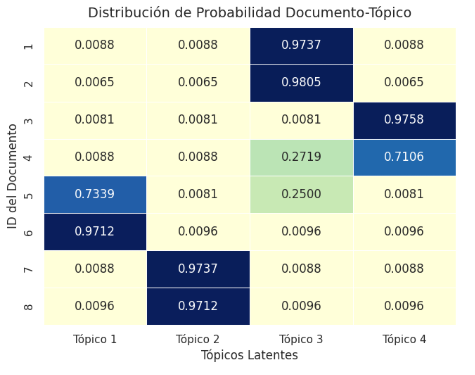
\includegraphics[keepaspectratio]{images/Captura de pantalla 2026-05-21 122847.png}}

Entre el texto 4 y 5, el modelo estaba 70\% seguro (aprox) de que los
textos pertenecían a su tópico asignado. Por compartir algunas palabras,
el modelo estaba 20\% seguro (aprox) de que pertenecían a otro tópico.

Para ver más de este fenómeno de inseguridad, puede ejecutarse el script
de python sobre nuestro dataset alternativo \texttt{data\_alt} ,ahí se
puede observar a un modelo que no está completamente seguro de a qué
tópico pertenecen los textos.

\subsection{Análisis de sentimientos}\label{anuxe1lisis-de-sentimientos}

{[}Steve{]}




\end{document}
